%% -*- coding: utf-8 -*-
\documentclass[12pt,pagesize,paper=landscape,paper=192mm:108mm]{scrbook} 
%1920x1080 1280x720
\areaset[current]{192mm}{108mm}
\usepackage{calc}
\usepackage[T2A]{fontenc}
\usepackage[utf8]{inputenc}
\usepackage[english,russian]{babel}
\usepackage{microtype}
\usepackage{misccorr}
\usepackage{cmap}
%\usepackage[unicode=true]{hyperref}
\usepackage{graphicx}
\usepackage{amssymb}
\usepackage{amsmath}
%\usepackage{srcltx}
\usepackage{textcomp}
\usepackage{xspace}
%научные символы и смайлики \smiley \frownie
\usepackage{wasysym}
\usepackage{ccicons}
\begin{document}
\begin{titlepage}
  \vspace*{-0.5em}
  \begin{center}    
    \hspace*{3em}
    \begin{minipage}[t]{3em}
      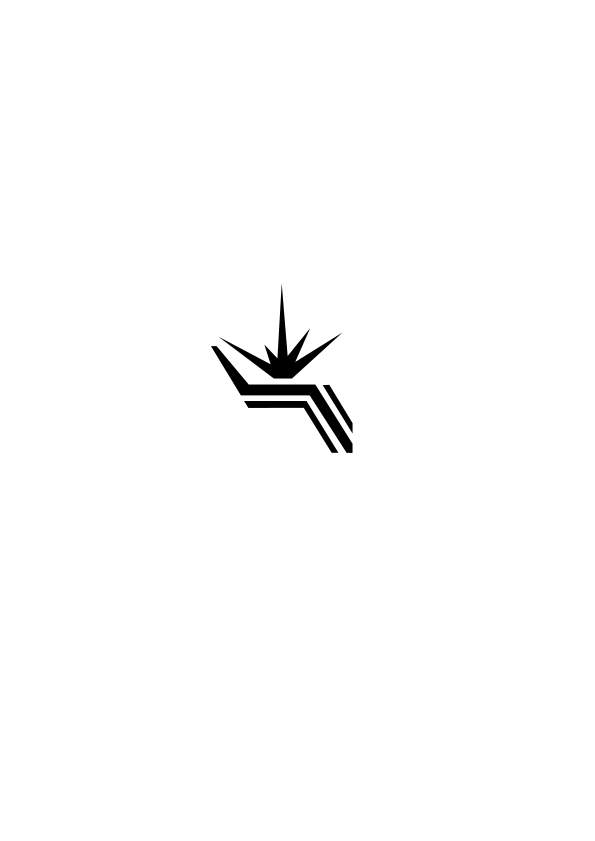
\includegraphics[width=\textwidth]{../BINP-logo}
    \end{minipage}\hfill
    \begin{minipage}{0.23\linewidth}
    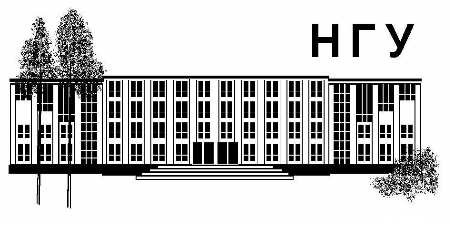
\includegraphics[width=\textwidth]{../NSU-logo}
    \end{minipage}
    \hfill
    \hspace*{6em}

    Кафедра теоретической физики физического факультета НГУ
    \medskip

    \Large
    Профессор Черняк В.\,Л.
    \bigskip

    \huge
    \textbf{Теория электрослабых взаимодействий}
    \bigskip

    \Large
    Лекция № 13
    \vfill

\normalsize    Новосибирск 2013
  \smallskip

  \ccbysa
  \end{center}
\end{titlepage}
\newpage

\vspace*{-1em}
\begin{center}
 \vfill
  \begin{minipage}{0.66\linewidth}
    Полулептонный распад $B\to\pi^0\ell\bar{\nu}_{\ell}$.  Физический
    смысл формфакторов адронных матричных элементов. Бета"=распад
    нейтрона: $n\to p e^-\bar{\nu}_e$.  Анализ адронного матричного
    элемента: 4 формфактора, относительный вклад разных формфакторов,
    разложение их в~нуле.  Вычисление $f_1(0)=1$ с использованием
    изотопической симметрии.  Правила сумм Адлера для нахождения
    $g_1(0)$. Константа $g_{\pi NN}$.  Вывод соотношения
    Голдбергера"=Треймана (связь $g_1(0)$, $g_{\pi NN}$ и $f_{\pi}$)
    дивергенция аксиального тока и связь $g_1(q^2)$ и $g_2(q^2)$ в
    киральном $SU(2)$ пределе, полюсной вклад $\pi$"=мезона в
    формфактор $g_2(q^2)$ при~вычислении аксиальной части адронного
    матричного элемента.
  \end{minipage}
  \vfill
  % Новосибирск 2013

  % \normalsize \ccbysa
\end{center}
\end{document}
